\begin{frame}[c]
    \frametitle{基于铌酸锂的可编程多波长可调谐滤波器设计:概述}
    \begin{columns}
        \begin{column}{.6\textwidth}
            \begin{itemize}
                \item Yao, Y.;  Hou, J.;  Liu, H.;  Zhang, A.;  Liu, B.;  Zhang, H.; Liu, J., Design of \textcolor{purple}{programmable} multi-wavelength tunable filter on \textcolor{red}{lithium niobate}. Results in Physics 2019, 15, 102741.
                \item \textcolor{blue}{创新点:}通过对电极对进行编码,实现了谐振波长数和波长间距的可编程化。
                \item \textcolor{blue}{瓶颈:}工作波段过窄(文章中展示的只有几个 $\mathrm{nm}$)。
                \item \textcolor{blue}{意义:}可以应用于开发具有快速调谐速度的基于铌酸锂的单芯片。
            \end{itemize}
        \end{column}
        \begin{column}{.4\textwidth}
            \begin{figure}[H] %H为当前位置,!htb为忽略美学标准,htbp为浮动图形
                \centering %图片居中
                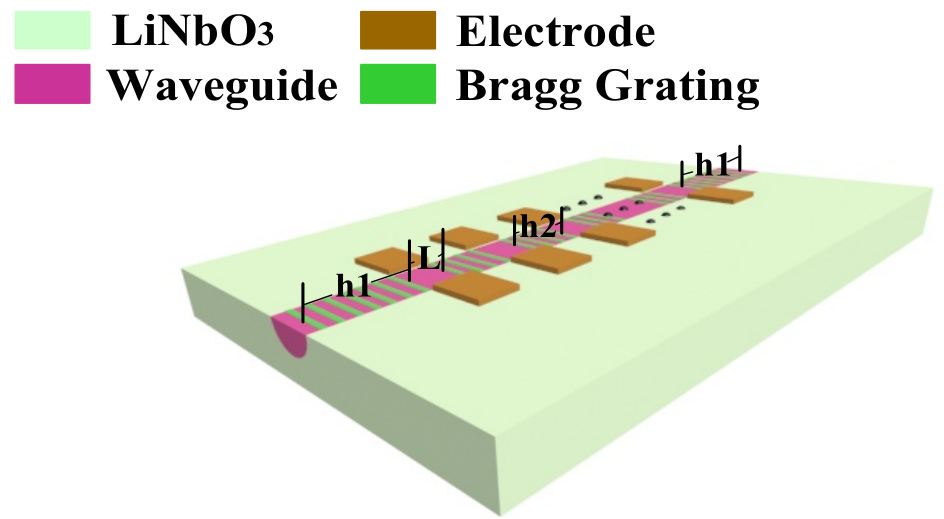
\includegraphics[width=1.\textwidth]{figures/Design of programmable multi-wavelength tunable filter on lithium niobate_1.png} %插入图片,[]中设置图片大小,{}中是图片文件名
                \caption{器件示意图}
            \end{figure}
        \end{column}
    \end{columns}

    \begin{itemize}
        \item 原理:光通过每个宽为 $L$ 的波导会产生相移\[\varphi=\frac{4\pi}{\lambda}(n_{\mathrm{eff}}-\frac{\gamma_{33}n_{\mathrm{eff}}^3V\Gamma}{2d})L\]通过改变 $V$ 来调整目标波长
    \end{itemize}
\end{frame}

\begin{frame}[c]
    \frametitle{基于铌酸锂的可编程多波长可调谐滤波器设计:滤波性能}

    波长选择性较好,透射峰极尖锐,但是工作波长太窄:

    \begin{columns}
        \begin{column}{0.5\textwidth}
            \begin{figure}[H] %H为当前位置,!htb为忽略美学标准,htbp为浮动图形
                \centering %图片居中
                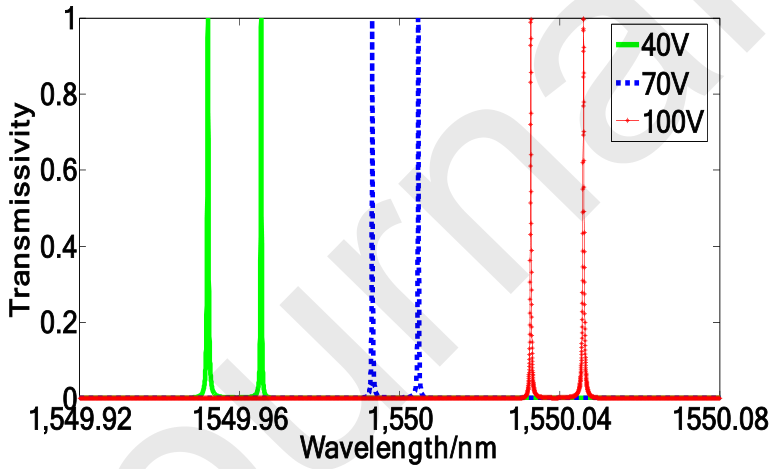
\includegraphics[width=.9\textwidth]{figures/Design of programmable multi-wavelength tunable filter on lithium niobate_2.png} %插入图片,[]中设置图片大小,{}中是图片文件名
            \end{figure}
            \begin{figure}[H] %H为当前位置,!htb为忽略美学标准,htbp为浮动图形
                \centering %图片居中
                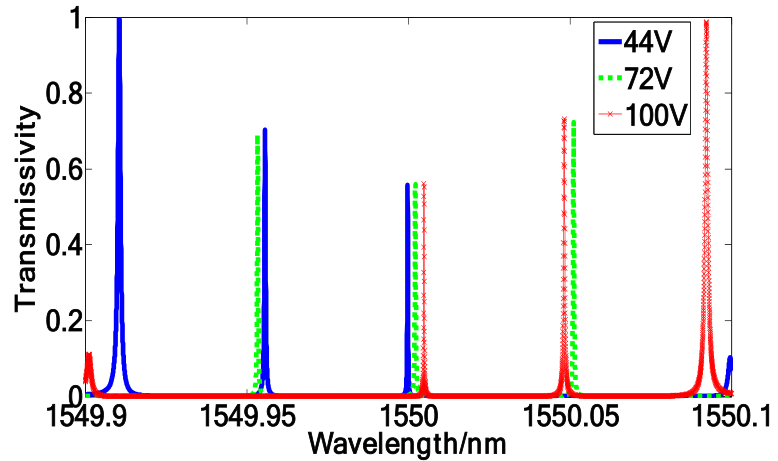
\includegraphics[width=.9\textwidth]{figures/Design of programmable multi-wavelength tunable filter on lithium niobate_3.png} %插入图片,[]中设置图片大小,{}中是图片文件名
                \caption{改变电压 $V$ 的效果}
            \end{figure}
        \end{column}
        \begin{column}{0.5\textwidth}
            \begin{figure}[H] %H为当前位置,!htb为忽略美学标准,htbp为浮动图形
                \centering %图片居中
                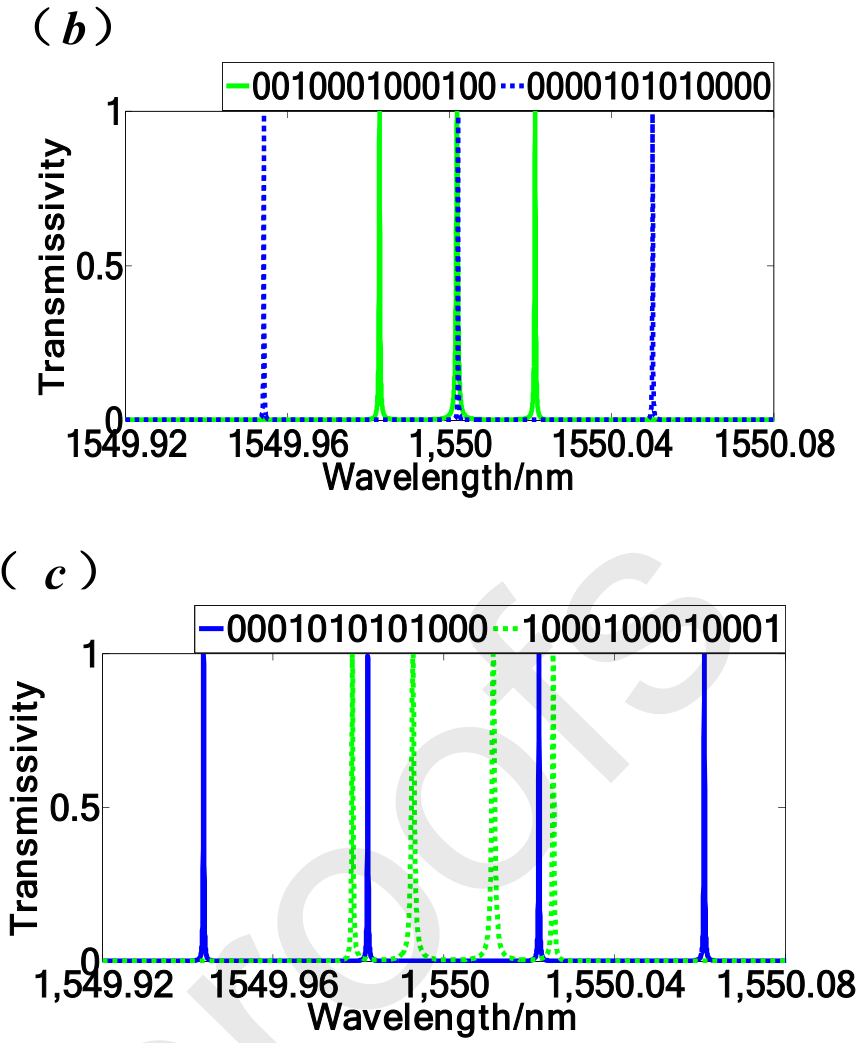
\includegraphics[width=.9\textwidth]{figures/Design of programmable multi-wavelength tunable filter on lithium niobate_4.png} %插入图片,[]中设置图片大小,{}中是图片文件名
                \caption{上面的编码指的是“第几个波导加电压”}
            \end{figure}
        \end{column}
    \end{columns}

\end{frame}